\documentclass[tikz,border=8pt]{standalone}
\usepackage{tikz}
\usetikzlibrary{arrows.meta, positioning, shapes.geometric}

\begin{document}

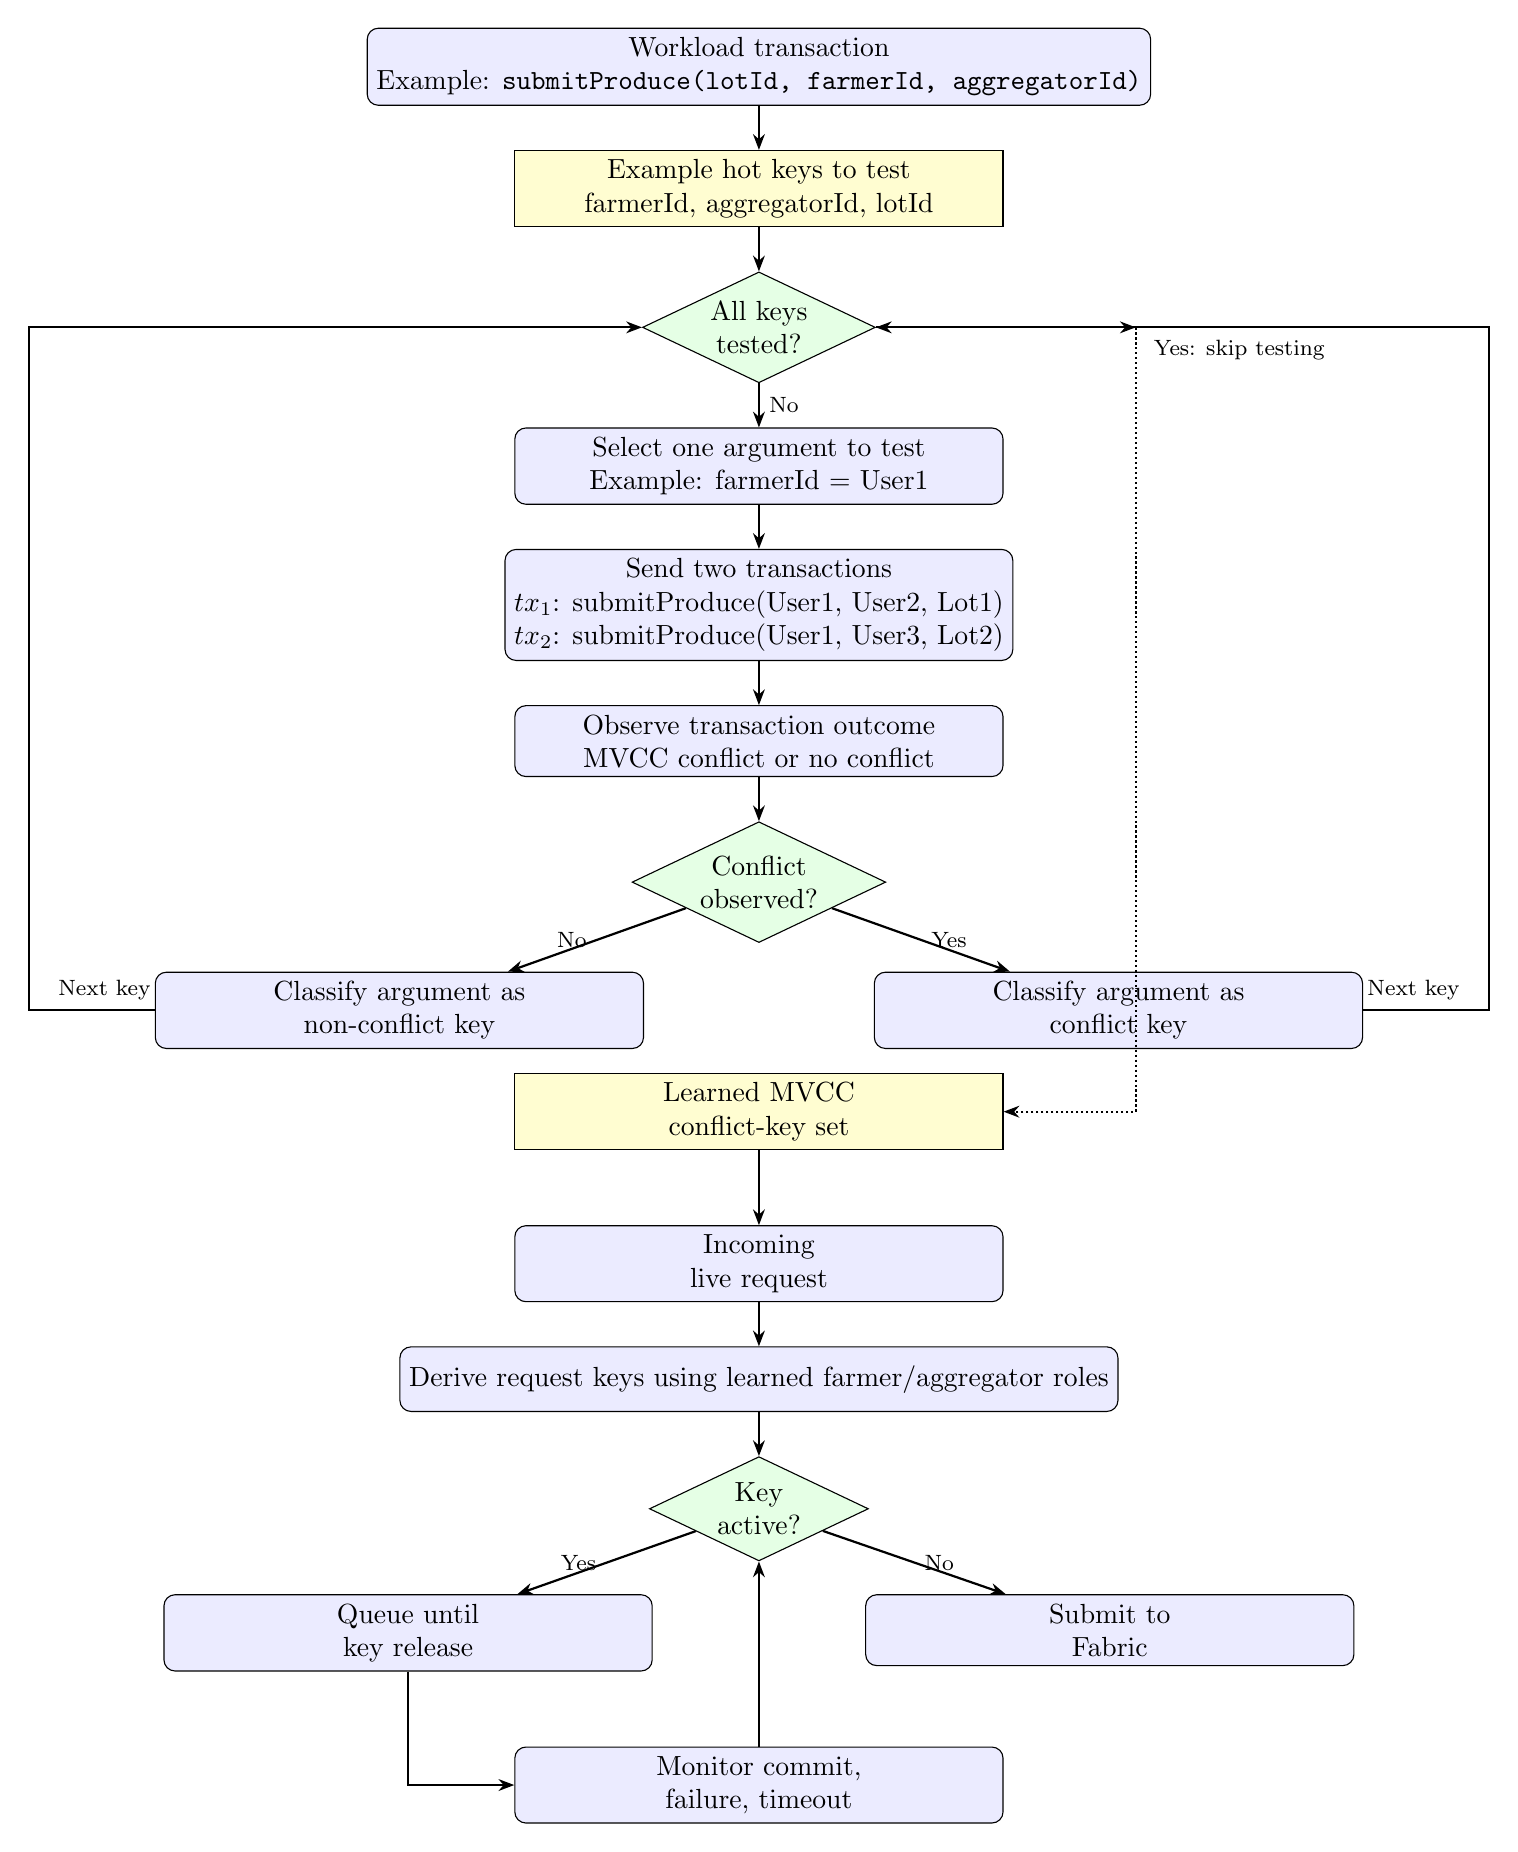
\begin{tikzpicture}[
    node distance=0.56cm,
    stage/.style={rectangle, draw, rounded corners, align=center, minimum width=6.2cm, minimum height=0.82cm, fill=blue!8},
    store/.style={rectangle, draw, align=center, minimum width=6.2cm, minimum height=0.82cm, fill=yellow!18},
    decision/.style={diamond, draw, align=center, aspect=2.1, inner sep=1.5pt, minimum width=2.7cm, fill=green!10},
    arrow/.style={-{Stealth[length=2mm]}, thick}
]
\node[stage] (req) {Workload transaction\\Example: \texttt{submitProduce(lotId, farmerId, aggregatorId)}};
\node[store, below=of req] (hotkeys) {Example hot keys to test\\farmerId, aggregatorId, lotId};
\node[decision, below=of hotkeys] (alltested) {All keys\\tested?};
\node[stage, below=of alltested] (args) {Select one argument to test\\Example: farmerId = User1};
\node[stage, below=of args] (pairwise) {Send two transactions\\$tx_1$: submitProduce(User1, User2, Lot1)\\$tx_2$: submitProduce(User1, User3, Lot2)};
\node[stage, below=of pairwise] (observefail) {Observe transaction outcome\\MVCC conflict or no conflict};
\node[decision, below=of observefail] (conflict) {Conflict\\observed?};
\node[stage, below left=0.75cm and 0.65cm of conflict] (nonconflict) {Classify argument as\\non-conflict key};
\node[stage, below right=0.75cm and 0.65cm of conflict] (conflictkey) {Classify argument as\\conflict key};
\node[store, below=1.65cm of conflict] (learned) {Learned MVCC\\conflict-key set};

\node[stage, below=0.95cm of learned] (live) {Incoming\\live request};
\node[stage, below=of live] (map) {Derive request keys using learned farmer/aggregator roles};
\node[decision, below=of map] (active) {Key\\active?};
\node[stage, below left=0.75cm and 0.65cm of active] (queue) {Queue until\\key release};
\node[stage, below right=0.75cm and 0.65cm of active] (fabric) {Submit to\\Fabric};
\node[stage, below=2.35cm of active] (monitor) {Monitor commit,\\failure, timeout};

\draw[arrow] (req) -- (hotkeys);
\draw[arrow] (hotkeys) -- (alltested);
\draw[arrow] (alltested) -- node[right, font=\footnotesize]{No} (args);
\draw[arrow] (alltested.east) -- ++(3.3cm,0) coordinate (skipturn);
\node[right, font=\footnotesize] at ([xshift=3pt,yshift=-8pt]skipturn) {Yes: skip testing};
\draw[arrow, densely dotted] (skipturn) |- (learned.east);
\draw[arrow] (args) -- (pairwise);
\draw[arrow] (pairwise) -- (observefail);
\draw[arrow] (observefail) -- (conflict);
\draw[arrow] (conflict) -- node[left, font=\footnotesize]{No} (nonconflict);
\draw[arrow] (conflict) -- node[right, font=\footnotesize]{Yes} (conflictkey);
\draw[arrow] (nonconflict.west)  -| ++(-1.6cm,0) node[above, font=\footnotesize, pos=0.2]{Next key} |- (alltested.west);
\draw[arrow] (conflictkey.east)  -| ++(1.6cm,0) node[above, font=\footnotesize, pos=0.2]{Next key} |- (alltested.east);
\draw[arrow] (learned) -- (live);
\draw[arrow] (live) -- (map);
\draw[arrow] (map) -- (active);
\draw[arrow] (active) -- node[left, font=\footnotesize]{Yes} (queue);
\draw[arrow] (active) -- node[right, font=\footnotesize]{No} (fabric);
\draw[arrow] (queue.south) |- (monitor.west);

\draw[arrow] (monitor.north) -- (active.south);
\end{tikzpicture}

\end{document}
